\documentclass[12pt,a4paper]{article}
\usepackage[utf8]{inputenc}
\usepackage[spanish]{babel}
\usepackage{amsmath}
\usepackage{amsfonts}
\usepackage{amssymb}
\usepackage{geometry}
\usepackage{listings}
\usepackage{xcolor}
\usepackage{graphicx}
\usepackage{float}
\geometry{margin=2.5cm}

% Configuración de listings para código R
\lstset{
    basicstyle=\ttfamily\small,
    breaklines=true,
    breakatwhitespace=true,
    frame=single,
    language=R,
    showstringspaces=false,
    columns=flexible
}

\title{Estadística y Diseño de Experimentos\\
Ejercicios 2}
\date{13 de Junio, 2025}
\author{}

\begin{document}

\maketitle

\noindent\textbf{Nombre del alumnx:} \underline{\hspace{0.5cm}Martínez Buenrostro Jorge Rafael\hspace{0.5cm}}

\vspace{1cm}

En la fabricaci\'on de un motor se deben unir dos tipos de propulsores (tipo 1 y tipo 2). Se sospecha que la resistencia al corte de esta uni\'on est\'a relacionada con la edad (en semanas) del lote de propulsores del tipo 1. En la siguiente tabla se muestra la Resistencia al corte (medida en psi) y la Edad (en semanas) del lote del propulsor tipo 1.

\begin{enumerate}
  \item Identifique qui\'en es la variable de respuesta \textit{Y} y qui\'en es la variable regresora \textit{X} y escriba el modelo de regresi\'on.
  \\
  La variable de respuesta \textit{Y} es la Resistencia al corte (medida en psi) y la variable regresora \textit{X} es la Edad (en semanas) del lote del propulsor tipo 1. El modelo de regresi\'on es:
  \[ Resistencia = \beta_0 + \beta_1 Edad + \epsilon \]
  
  \item Grafique el diagrama de dispersi\'on de los datos.
  \begin{figure}[H]
    \centering
    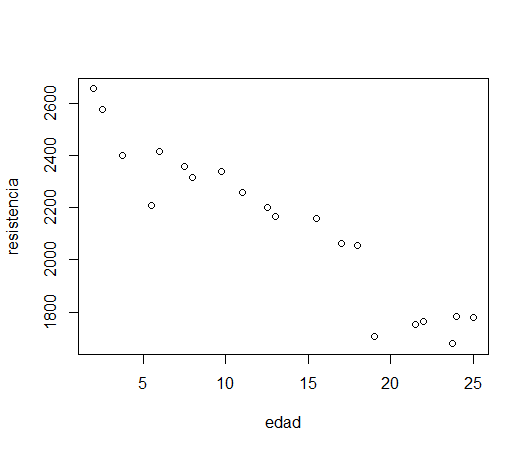
\includegraphics[width=0.6\textwidth]{img/DiagramaDispersion.png}
  \end{figure}
  
  \newpage

  \item Obtenga los estimadores para $\beta_0$ y $\beta_1$ y escriba la ecuaci\'on de la recta ajustada.
  \begin{lstlisting}
    lm(resistencia~edad)
    modelo<-lm(resistencia~edad)
    abline(modelo)
    summary(modelo)
  \end{lstlisting}
  Para obtener los estimadores de $\beta_0$ y $\beta_1$, se puede utilizar la funci\'on \texttt{lm()} y la funci\'on \texttt{summary()} en R. Los resultados son: $\beta_0=2627.82$ y $\beta_1=-37.154$, y la ecuaci\'on de la recta ajustada es:
    \[ Resistencia = 2627.82 - 37.15*Edad \]

  \item Grafique la recta de la regresi\'on junto con los datos. ¿Qu\'e tan bueno cree que es el ajuste? El ajuste parece ser bueno, ya que la recta de regresi\'on pasa cerca de la mayor\'ia de los puntos del diagrama de dispersi\'on.
  \begin{figure}[H]
    \centering
    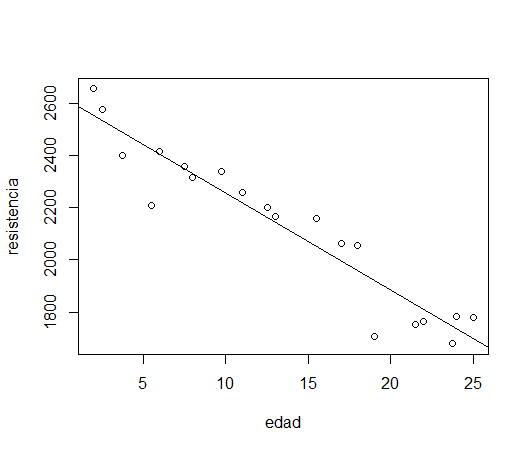
\includegraphics[width=0.7\textwidth]{img/RectaRegresion.png}
  \end{figure}

  \item Efect\'ue la prueba de significancia de la regresi\'on para un nivel $\alpha=0.05$. Escriba el valor del p-valor. ¿Qu\'e conclusiones puede hacer sobre $\beta_1$?
  \\ 
  La prueba de significancia consiste en comparar el p-valor con $\alpha$. Si el p-valor es menor que $\alpha$ se rechaza la hip\'otesis nula. En este caso, el p-valor lo obtenemos de la funci\'on \texttt{summary()}, y es de $1.64e-10$. Como $1.64e-10 < 0.05$, se rechaza la hip\'otesis nula y se concluye que $\beta_1$ es significativamente diferente de cero, lo que indica que la edad del lote del propulsor tipo 1 tiene un efecto significativo en la resistencia al corte.
  \newpage

  \item Suponga que se tienen tres lotes del propulsor tipo 1, con 5, 10 y 15 semanas de edad respectivamente. ¿Cu\'al es la estimaci\'on para la resistencia seg\'un el modelo de regresi\'on (para cada lote)?
  \begin{lstlisting}
    > predict(modelo, list(edad=c(5)), interval = 'prediction')
        fit      lwr      upr
    1 2442.054 2229.021 2655.087
    > predict(modelo, list(edad=c(10,15)), interval = 'prediction')
        fit      lwr      upr
    1 2256.286 2048.385 2464.188
    2 2070.518 1863.382 2277.655
  \end{lstlisting}
  La estimaci\'on para la resistencia seg\'un el modelo de regresi\'on es:
  \begin{itemize}
    \item Para 5 semanas de edad: 2442.054 psi
    \item Para 10 semanas de edad: 2256.286 psi
    \item Para 15 semanas de edad: 2070.518 psi
  \end{itemize}

  \item Calcule el valor del coeficiente de determinaci\'on (Multiple R Squared). Seg\'un este coeficiente. ¿qu\'e tan bueno es el ajuste de la regresi\'on?
  \\
  El valor del coeficiente de determinaci\'on (Multiple R Squared) se obtiene de la funci\'on \texttt{summary()} y es de $0.9018$. Esto indica que el 90.18\% de la variabilidad en la resistencia al corte puede ser explicada por la edad del lote del propulsor tipo 1, lo que sugiere que el ajuste de la regresi\'on es bueno.
  
  \item VERIFICACI\'ON DE SUPUESTOS DEL MODELO. (Obtenga primero los residuales)
  \\
  Para obtener los residuales se puede utilizar la funci\'on \texttt{rstudent()} o la funci\'on \texttt{residuals()} en R. Para este caso, se utilizar\'a la funci\'on \texttt{rstudent()}.
  \begin{enumerate}
    \item NORMALIDAD. Grafique los residuales contra los cuantiles de una normal (qqnorm,qqline). ¿Se satisface este supuesto? Si, se satisface este supuesto, ya que los puntos se encuentran cerca de la l\'inea recta.
    \begin{figure}[H]
      \centering
      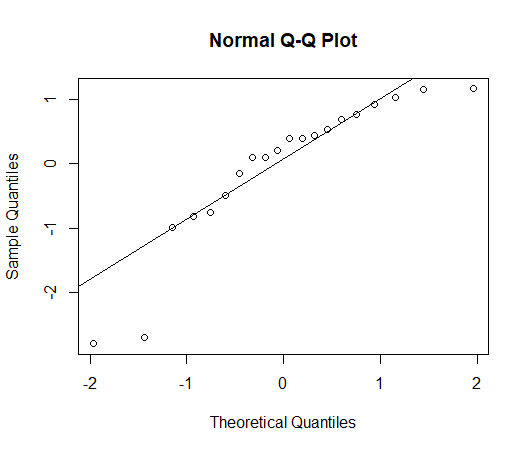
\includegraphics[width=0.6\textwidth]{img/Normalidad.png}
    \end{figure}

    \item MEDIA CERO, VARIANZA CONSTANTE E INDEPENDENCIA. Grafique los residuales contra los predichos para verificar los tres supuestos (predict, rstudent).
    \begin{figure}[H]
      \centering
      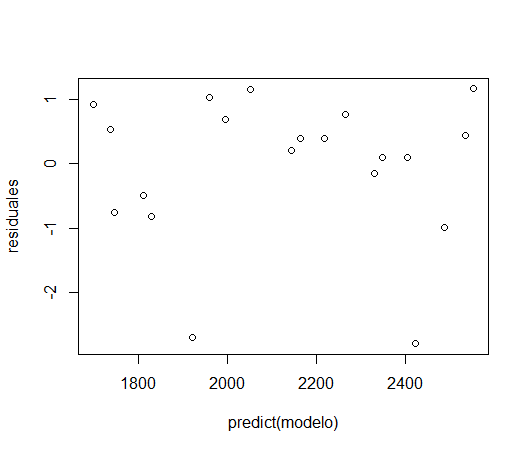
\includegraphics[width=0.6\textwidth]{img/MediaVarianzaIndependencia.png}
    \end{figure}
  ¿Observa alguna anomal\'ia? No, ya que lo datos se encuentran distribuidos aleatoriamente alrededor de cero (media igual a 0 y errores independientes) y se pueden delimitar dos bandas paralelas (varianza constante). 
  \end{enumerate}
  
  \item PUNTOS AT\'IPICOS E INFLUYENTES.
  \begin{enumerate}
    \item Utilizando la gr\'afica anterior, ¿se observan puntos que puedan considerarse como at\'ipicos (outliers)? Si, hay dos puntos que pueden considerarse como at\'ipicos, ya que se encuentran fuera de las bandas paralelas.
  
    \item Utilizando la distancia de Cook, verifique si hay puntos inlfuyentes.
    \\
    Para poder calcalar la distancia de Cook, se puede utilizar la funci\'on \texttt{cooks.distance()} en R. Si alg\'un dato tiene una distancia de Cook mayor a 1, se considera un punto influyente.
    \begin{lstlisting}
    > cooks.distance(modelo)
              1            2            3            4            5 
    0.0373281981 0.0497291858 0.0010260760 0.0161482719 0.3343768993 
              6            7            8            9           10 
    0.2290842436 0.0270491200 0.0191323748 0.0003959877 0.0047094549 
              11           12           13           14           15 
    0.0012482345 0.0761514881 0.0889892211 0.0192517639 0.0166302585 
              16           17           18           19           20 
    0.0387158541 0.0005955991 0.0041888627 0.1317143774 0.0425721512 
    > cooks.distance(modelo)>1
        1     2     3     4     5     6     7     8     9    10    11
    FALSE FALSE FALSE FALSE FALSE FALSE FALSE FALSE FALSE FALSE 
      12    13    14    15    16    17    18    19    20 
    FALSE FALSE FALSE FALSE FALSE FALSE FALSE FALSE FALSE
    \end{lstlisting}
  \end{enumerate}

  \item Escriba una conclusi\'on general para este problema.
  \\
  Los resultados del an\'alisis de regresi\'on indican que existe una relaci\'on significativa entre la edad del lote del propulsor tipo 1 y la resistencia al corte. El modelo de regresi\'on lineal ajustado sugiere que a medida que aumenta la edad del lote, la resistencia al corte disminuye. El coeficiente de determinaci\'on indica que el modelo explica una gran parte de la variabilidad en la resistencia al corte. Los supuestos del modelo parecen cumplirse adecuadamente, y no se identificaron puntos influyentes significativos. En general, se puede concluir que la edad del lote del propulsor tipo 1 es un factor importante a considerar en la fabricaci\'on de motores para asegurar una resistencia adecuada al corte.
\end{enumerate}

\newpage
\section*{C\'odigo en R}

\begin{lstlisting}
  > #Carga de datos
> resistencia <- c(2158.70, 1678.15, 2316.00, 2061.30, 2207.50, 1708.30, 1784.70, 
+                  2575.00, 2357.90, 2256.70, 2165.20, 2399.55, 1779.80, 2336.75, 
+                  1765.30, 2053.50, 2414.40, 2200.50, 2654.20, 1753.70)
> edad <- c(15.50, 23.75, 8.00, 17.00, 5.50, 19.00, 24.00, 2.50, 7.50, 11.00, 
+           13.00, 3.75, 25.00, 9.75, 22.00, 18.00, 6.00, 12.50, 2.00, 21.50)
> 
> 
> # 1. Identificar variables
> # Variable de respuesta Y: Resistencia
> # Variables regresora: Edad
> # Modelo: Y = B0 + B1X + d
> 
> 
> # 2. Diagrama de dispersion de los datos
> plot(edad,resistencia)
> 
> # 3. Estimadores para B0 y B1
> lm(resistencia~edad)

Call:
lm(formula = resistencia ~ edad)

Coefficients:
(Intercept)         edad  
    2627.82       -37.15  

>
> modelo<-lm(resistencia~edad)
> abline(modelo)
> summary(modelo)

Call:
lm(formula = resistencia ~ edad)

Residuals:
    Min      1Q  Median      3Q     Max 
-215.98  -50.68   28.74   66.61  106.76 

Coefficients:
            Estimate Std. Error t value Pr(>|t|)    
(Intercept) 2627.822     44.184   59.48  < 2e-16 ***
edad         -37.154      2.889  -12.86 1.64e-10 ***
---
>
> # Ecuacion de la recta ajustada
> cat("Resistencia =", round(beta0, 2), "+", round(beta1, 2), "* Edad\n")
Error: objeto 'beta0' no encontrado

> cat("Resistencia =", round(coef(modelo)[1], 2), "+", round(coef(modelo)[2], 2), "* Edad\n")
Resistencia = 2627.82 + -37.15 * Edad
> 
> # 4. Grafica de la recta de regresion con datos
> plot(edad,resistencia)
> abline(modelo)
> 
> 
> # 5. Prueba de significancia, p-valor<alpha
> # p-valor = 1.64e-10
> # alpha = 0.05
> 
> 
> # 6. Estimacion para lotes tipo 1 con 5, 10 y 15
> predict(modelo, list(edad=c(5)), interval = 'prediction')
       fit      lwr      upr
1 2442.054 2229.021 2655.087
> predict(modelo, list(edad=c(10,15)), interval = 'prediction')
       fit      lwr      upr
1 2256.286 2048.385 2464.188
2 2070.518 1863.382 2277.655
> 
> 
> # 7. Coeficiente de determinacion
> # Multiple R-squared: 0.9018
> 
> # 8. Verificacion de supuestos del modelo
> residuales<-residuals(modelo)
> residuales<-rstudent(modelo)
> qqnorm(residuales)
> plot(predict(modelo),residuales)
> 
> 
> # 9. Puntos atipicos e influyentes
> cooks.distance(modelo)
           1            2            3            4            5 
0.0373281981 0.0497291858 0.0010260760 0.0161482719 0.3343768993 
           6            7            8            9           10 
0.2290842436 0.0270491200 0.0191323748 0.0003959877 0.0047094549 
          11           12           13           14           15 
0.0012482345 0.0761514881 0.0889892211 0.0192517639 0.0166302585 
          16           17           18           19           20 
0.0387158541 0.0005955991 0.0041888627 0.1317143774 0.0425721512 
> cooks.distance(modelo)>1
    1     2     3     4     5     6     7     8     9    10    11    12 
FALSE FALSE FALSE FALSE FALSE FALSE FALSE FALSE FALSE FALSE FALSE FALSE 
   13    14    15    16    17    18    19    20 
FALSE FALSE FALSE FALSE FALSE FALSE FALSE FALSE 
> outliers<-which(abs(residuales) > 2)
> if(length(outliers) > 0) {
+     print(outliers)
+ } else {
+     cat("No se detectaron outliers significativos\n")
+ }
5 6 
5 6 
>
\end{lstlisting}

\end{document}